%-------------------------------------------------------------------------------
%-------------------------------------------------------------------------------
\section{Intégrales}
%-------------------------------------------------------------------------------

% Jacobien et changement de variables en dimension supérieure ou égale à 2.

% \begin{theorem}{Fubini-Tonelli}
% \end{theorem}
% 
% \begin{theorem}{Fubini-Lebesque}
% \end{theorem}

%-------------------------------------------------------------------------------
\subsection{Difféomorphisme}
%-------------------------------------------------------------------------------

\begin{definition}[Difféomorphisme]
  Soient $\Xcal$ et $\Ycal$ deux ouverts de $\Rbb^n$ et une bijection $g : \Xcal \mapsto \Ycal$. $g$ est un difféomorphisme si $g$ est différentiable partout dans $\Xcal$ et que $g^{-1}$ est différentiable partout dans $\Ycal$. \\
  Si, de plus, les dérivées partielles de $g$ et $g^{-1}$ sont partout continues, $g$ est un $C^1$-difféomorphisme.
\end{definition}

%-------------------------------------------------------------------------------
\paragraph*{Différentielle de la réciproque.}
Si $g : \Xcal \mapsto \Ycal$ est un difféomorphisme, puisque $g^{-1} \circ g = Id$ et que $D_x Id = I_n$, on a
$$
I_n = D_x(g^{-1} \circ g) = D_{g(x)}(g^{-1}) D_x g 
\qquad \text{(par composition)},
$$
soit
$$
D_{g(x)}\left(g^{-1}\right) = (D_x g)^{-1}.
$$
On retrouve ainsi la formule valable dans $\Rbb$ :
$$
(g^{-1})'(y) = 1 /g'(x)
\qquad \text{ou} \quad x = g^{-1}(y).
$$

\begin{theorem}[Inversion globale]
  Soit $\Xcal$ un ouvert de $\Rbb^n$ et $g : \Xcal \mapsto \Rbb^n$. Supposons que $g$ est injective, différentiable sur tout $\Xcal$ et que ses dérivées partielles sont partout continues dans $\Xcal$. Si, de plus, $D_x g$ est inversible sur tout $\Xcal$, alors $g : \Xcal \mapsto \Ycal = g(\Xcal)$ est un $C^1$-difféomorphisme.
\end{theorem}

\proof Non démontré. \eproof

\remark
Ce théorème assure le $C^1$-difféomorphisme sans exiger la différentiabilité continue de $g^{-1}$.

%-------------------------------------------------------------------------------
\subsection{Jacobien, changement de variable}
%-------------------------------------------------------------------------------

\begin{definition}[Jacobien]
  Pour $g : \Rbb^n \mapsto \Rbb^n$, le jacobien de $f$ au point $x$ est le déterminant de sa matrice jacobienne au point $x$ : 
  $$
  |J_x f|.
  $$
\end{definition}

\remark
Le jacobien d'un difféomorphisme ne peut pas être nul, puisqu'un difféomorphisme est bijectif :
$$
|J_x f| \neq 0.
$$

\begin{theorem}[Changement de variable]
  Soit $\Xcal$ et $\Ycal$ deux ouverts de $\Rbb^n$ et $g : \Xcal \mapsto \Ycal = g(\Xcal)$ un $C^1$-difféomorphisme et $f : \Ycal \mapsto \Rbb^+$, on a 
  $$
  \int_\Ycal f(y) \; \d y = \int_\Xcal f \circ g(x) |J_x g| \; \d x.
  $$
\end{theorem}

\proof
Non démontrée.
% : la preuve passe par le découpage du domaine d'intégration en fonction des différents type d'action de la matrice jacobienne $J_x g$ (transvection, permutation ou dilatation).
\eproof

%-------------------------------------------------------------------------------
\textcolor{gray}{\remark
La contrainte de signe pour $f$ assure que le résultat de l'intégration ne dépend pas de l'ordre selon lequel on intègre par rapport aux différente coordonnée (théorème Fubini-Tonelli). Le théorème de Fubini-Lebesgue lève cette contrainte mais requiert que $f$ soit bornée.}

%-------------------------------------------------------------------------------
\begin{corollary*}[Coordonnées polaires]
  Pour tout $f : \Rbb^2 \mapsto \Rbb^+$, 
  $$
  \int_\Rbb \int_\Rbb f(x, y) \; \d x \d y
  = \int_{\Rbb^+} \int_0^{2 \pi} f(\rho \cos \theta, \rho \sin \theta) \rho \; \d \rho \d \theta
  $$
\end{corollary*}

\proof
\begin{itemize}
  \item On a vu que la transformation en coordonnées polaires $g$ est partout différentiable et que $|J_{(\rho, \theta)}g| = \rho$.
  \item On vérifie facilement que $g$ est bijective et que ses dérivées partielles sont partout continues.
\end{itemize}
\eproof

%-------------------------------------------------------------------------------
\exemple{
  Pour calculer 
  $$
  I = \int_\Rbb e^{-x^2} \; \d x,
  $$
  on peut passer en coordonnées polaires pour calculer
  \begin{align*}
  J 
  & = \int_\Rbb \int_\Rbb e^{-(x^2+y^2)} \; \d x \; \d y
  = \int_{\Rbb^+} \int_0^{2 \pi} e^{-\rho^2} \rho \; \d \rho \; \d \theta \\
  & = \int_{\Rbb^+} e^{-\rho^2} \rho \; \d \rho \times \int_0^{2 \pi} \d \theta 
  = \left[-\frac12 e^{-\rho^2}\right]_0^\infty \times 2 \pi \\
  & = \pi
  \end{align*}
  puis remarquer que $J = I^2$ pour conclure que $I = \sqrt{\pi}$.
}

\remark
Par le le même calcul, on montre que $\int_\Rbb e^{-x^2/2} \; \d x = \sqrt{2 \pi}$, ce qui justifie la constante de normalisation de la densité de la loi normale d'espérance nulle et de variance 1 : 
$$
\phi(x) = \frac1{\sqrt{2\pi}} \exp(- x^2/2).
$$

%-------------------------------------------------------------------------------
%-------------------------------------------------------------------------------
\section{Extremums}
%-------------------------------------------------------------------------------

%-------------------------------------------------------------------------------
\subsection{\textcolor{gray}{Variétés}}
%-------------------------------------------------------------------------------

\textcolor{gray}{Courbe de niveau (cf notes manuscrites, dans section chgt de variable)}

%-------------------------------------------------------------------------------
\subsection{Extremums}
%-------------------------------------------------------------------------------

\begin{definition}[Gradient]
  Soit $f : \Rbb^k \mapsto \Rbb$ différentiable en $x^*$, le gradient de $f$ en $x^*$ est le vecteur constitué de ses dérivées partielles évaluées en $x^*$ : 
  $$
  \nabla_{x^*}f 
  = \left[\begin{array}{c}
              \displaystyle{\left.\frac{\partial f}{\partial x_1}\right|_{x^*}}  \\
              \vdots \\
              \displaystyle{\left.\frac{\partial f}{\partial x_k}\right|_{x^*}} 
             \end{array}\right]
  = \left[J_{x^*} f\right]^\top.
  $$
\end{definition}

%-------------------------------------------------------------------------------
\remark
\begin{enumerate}
  \item Si $f$ est différentiable en $x$, on a
  $$
  f(x + h) = f(x) + \nabla_{x^*}f^\top h + o(\|h\|).
  $$
  \item Un point $x$ pour lequel le gradient de $f$ est nul est appelé {\em point stationnaire} (ou {\em point critique}) de $f$ : au premier ordre, la fonction $f$ est constante au voisinage de $x$.
\end{enumerate}


%-------------------------------------------------------------------------------
\begin{definition}[Matrice hessienne]
  Soit $f : \Rbb^n \mapsto \Rbb$ différentiable en $x^*$, la matrice hessienne ('la hessienne') $f$ en $x^*$ est la matrice ayant pour éléments génériques les dérivées secondes croisées évaluées en $x^*$ : 
  $$
  \nabla^2_{x^*}f 
  = \left[\left.\frac{\partial^2 f}{\partial x_i\partial x_j}\right|_{x^*} \right]_{1 \leq i, j \leq n}
%   = \left[\begin{array}{ccc}
%               \displaystyle{\left.\frac{\partial^2 f}{\partial x_1^2}\right|_{x^*}} & 
%               \cdots & 
%               \displaystyle{\left.\frac{\partial^2 f}{\partial x_1\partial x_k}\right|_{x^*}} \\
%               \vdots & 
%               \displaystyle{\left.\frac{\partial^2 f}{\partial x_i\partial x_j}\right|_{x^*}}\vdots & 
%               \\
%               \displaystyle{\left.\frac{\partial^2 f}{\partial x_k\partial x_1}\right|_{x^*}} & 
%               \cdots & 
%               \displaystyle{\left.\frac{\partial^2 f}{\partial x_k^2}\right|_{x^*}}
%           \end{array} \right].
  $$
  Les termes diagonaux de $\nabla^2_{x^*}f$ sont les dérivées secondes par rapport à chacune des coordonnées : 
  $$
  \left[ \nabla^2_{x^*}f \right]_{ii} 
  = \left.\frac{\partial^2 f}{\partial x_i^2}\right|_{x^*}.
  $$
  Notamment, si $f$ est $C^2$, $\nabla^2_{x^*}f$ est symétrique (car on peut alors inverser l'ordre des dérivées), ce qui implique qu'elle est diagonalisable.
\end{definition}

%-------------------------------------------------------------------------------
\begin{proposition} \label{prop:taylorOrdre2}
  Si $f$ est deux fois différentiable en $x$, alors
  $$
  f(x+h) = f(x) + \nabla_x f^\top \cdot h + \frac12 h^\top \cdot \nabla^2_x f \cdot h + o(\|h\|^2).
  $$
\end{proposition}

% {Démonstration de la proposition \ref{prop:taylorOrdre2}.}
\proof
  Pour alléger les notations, on note ici
  $$
  f'_i(x^*) = \left. \frac{\partial f}{\partial x_i}\right|_{x^*}, \qquad 
  f''_{ij}(x^*) = \left. \frac{\partial^2 f}{\partial x_i \partial x_j}\right|_{x^*}.
  $$
  La démonstration repose sur le développement de Taylor en 0 d'une fonction $\phi$ de $\Rbb$ dans $\Rbb$ deux fois différentiable qui vaut
  \begin{equation} \label{eq:taylor2phi}
  \phi(t) = \phi(0) + t \phi'(0) + \frac12 \phi''(0) + o(t^2).
  \end{equation}
  \begin{enumerate}
    \item On pose tout d'abord $h = t u$, où $u$ est un vecteur fixe et on définit la fonction 
    $$
      \begin{array}{rrcl}
        g : & \Rbb & \mapsto & \Rbb^n \\
        & t & \to & x + t u
      \end{array}
    $$
    qui vérifie
    $$
    J_t g = u.
    $$
    En posant $\phi = f \circ g$, on obtient ainsi
    $$
    f(x + h) = \phi(t).
    $$
    \item Il nous faut maintenant déterminer $\phi'(0)$ et $\phi''(0)$.
    \begin{description}
      \item[$\phi'(t)$:] on a
        $$
        \phi'(t) = J_t \phi 
        = J_{g(t)} f \cdot J_t g
        = \nabla_{g(t)}f^\top u
        = \sum_{i=1}^n u_i f'_i(g(t))
        $$
      \item[$\phi''(t)$:] on a
      $$
      \phi''(t) 
      = \frac{\partial}{\partial t} \phi'(t)
      = \sum_{i=1}^n u_i \frac{\partial}{\partial t} f'_i(g(t))
      $$
      puisque $u_i$ ne dépend pas de $t$. On remarque alors que
      $$
      J_x f_i' = [f''_{i1}(x) \; \dots \; f''_{in}(x)]
      $$
      donc
      $$
      \frac{\partial}{\partial t} f'_i(g(t)) 
      = J_{g(t)} f_i' \cdot J_t g
      = J_{g(t)} f_i' \cdot u
      = \sum_{j=1}^n u_j f''_{ij}(g(t)),
      $$
      soit
      $$
      \phi''(t) 
      = \sum_{i=1}^n u_i \sum_{j=1}^n u_j f''_{ij}(g(t))
      = u^\top \nabla_{g(t)} u.
      $$
    \end{description}
    En reportant dans l'équation \eqref{eq:taylor2phi}, on obtient
    \begin{align*}
      \phi(t) 
    %       & = \phi(0) + t \phi'(0) + \frac12 t^2 \phi''(0) + o(t^2) \\
      & = \phi(0) + t \nabla_{g(0)}f^\top u + \frac12 t^2 u^\top \nabla_{g(0)} u + o(t^2) \\
      & = \phi(0) + \nabla_{g(0)}f^\top h + \frac12 h^\top \nabla_{g(0)} h + o(t^2)
    \end{align*}
    car $h = tu$, soit, en utilisant $\phi(t) = f(x)$, $\phi(0) = f(x)$ et $g(0) = x$,
    $$
    f(x+h) 
    = f(x) + \nabla_{x}f^\top h + \frac12 h^\top \nabla_{x} h + o(t^2).
    $$
    \item Il reste à vérifier que $o(t^2) = o(\|h\|^2)$, ce qui est vrai car $\|h\|^2 = t^2 \|u\|^2$ et $\|u\|^2$ est constante.
  \end{enumerate}
\eproof

\remark
$f$ est deux fois différentiable en $x$ signifie que $f$ est différentiable en $x$ et que l'application $g$ de $\Rbb^k$ dans $\Rbb^k$ définie par $g(x) = \nabla_x f$ est elle-même différentiable en $x$.

\begin{definition}[Extremum local]
  Si $f$ est deux fois différentiable en $x$ et que son gradient y est nul : $\nabla_xf = 0$, alors
  \begin{itemize}
   \item $x$ est {\em maximum local} si $\nabla^2_x f$ est définie négative et
   \item $x$ est {\em minimum local} si $\nabla^2_x f$ est définie positive.
  \end{itemize}
  Dans les deux cas, $x$ est un {\em optimum relatif}.
\end{definition}

\remark
Puisque le gradient $\nabla_x f$ est nul, on a au voisinage de $x$ :
$$
f(x+h) - f(x) \simeq \frac12 h^\top \cdot \nabla^2_x f \cdot h.
$$
Un maximum (resp. minimum) se caractérise par le fait que la fonction $f$ diminue (resp. augmente) dans toutes les directions $h$. Le fait que $\nabla^2_x f$ soit définie négative (resp. positive) assure précisément que $f(x+h) - f(x)$ est négatif (resp. positif) dans tout le voisinage de $x$.

%-------------------------------------------------------------------------------
\subsection*{Cas de $f : \Rbb^2 \mapsto \Rbb$}
%-------------------------------------------------------------------------------

\begin{definition}[Notation de Monge]
  Pour $f : \Rbb^2 \mapsto \Rbb$, on note les dérivées au point $a = (x^*, y^*) \in \Rbb^2$
  \begin{align*}
    p & = \left.\frac{\partial f}{\partial x}\right|_a, &
    q & = \left.\frac{\partial f}{\partial y}\right|_a, &
    r & = \left.\frac{\partial^2 f}{\partial x^2}\right|_a, &
    s & = \left.\frac{\partial^2 f}{\partial x \partial y}\right|_a, &
    t & = \left.\frac{\partial^2 f}{\partial y^2}\right|_a
  \end{align*}
  c'est à dire
  $$
  \nabla_af = \left[\begin{array}{c} p \\ q \end{array} \right], 
  \qquad 
  \nabla^2_af = \left[\begin{array}{cc} r & s \\ s & t \end{array} \right].
  $$
\end{definition}

%-------------------------------------------------------------------------------
\paragraph*{Caractérisation des optimums.}
Toutes les valeurs propres d'une matrice définie positive ou négative sont de même signe. 
En dimension deux, cela signifie que leur produit (qui est égal au déterminant) est positif. Si le produit est positif, leur signe commun est donné par leur somme (qui est égale à la trace).

$a = (x^*, y^*)$ pour lequel $\nabla_a f = 0$ (i.e. $p = q = 0$) est donc
\begin{itemize}
  \item un optimum relatif de $f$ si 
  $$
  |\nabla^2_a f| = rt - s^2 > 0 ;
  $$
  \item un maximum relatif de $f$ si 
  $$
  |\nabla^2_a f| = rt - s^2 > 0 
  \qquad \text{et} \qquad
  \tr(\nabla^2_a f) = r + t < 0 ;
  $$
  \item un minimum relatif de $f$ si 
  $$
  |\nabla^2_a f| = rt - s^2 > 0 
  \qquad \text{et} \qquad
  \tr(\nabla^2_a f) = r + t > 0 ;
  $$
  \item un point selle de $f$ si 
  $$
  |\nabla^2_a f| = rt - s^2 < 0
  $$
  ($a$ est un maximum dans une direction et un minimum dans une autre).
\end{itemize}

% \progres{
%   Début Cours 7. Rappels :
%   \begin{enumerate}[\itemdot]
%     \item Changement de variables
%     $$
%     \int_{\Rbb^n} f(y) \; \d y = \int_{\Rbb^n} f \circ g (x) \; |J_x g| \; \d x
%     $$
%     $|J_x g| =$ jacobien de $g$ au point $x$.
%     \item Extrema
%     $$
%     f(x+h) = f(x) + (\nabla_x f)^\top h + \frac12 h^\top (\nabla^2_x f) h + o(\|h\|^2).
%     $$
%     $x =$ extremum local si $\nabla_x f = 0$, maximum si $\nabla^2_x f \preccurlyeq 0$, minimum si $\nabla^2_x f \succcurlyeq 0$.
%     \item Cas particulier $\Rbb^n = \Rbb^2$ : caractérisation des extrémum à partir du déterminant et de la trace de $\nabla^2_x f$.
%     \item Exercice maison.
%   \end{enumerate}
% }

\begin{exercise*}[A faire à la maison]
  Déterminer les points stationnaires de la fonction 
  $$
  f(x, y) = x^3 + y^3 - 3 xy
  $$
  déterminer s'il s'agit de maximums, de minimums ou de points selles.
\end{exercise*}

\solution{
  \begin{description}
    \item[Points critiques :] Le gradient de $f$ vaut
    $$
    \nabla f = \left[\begin{array}{c} 3x^2 - 3y \\ 3y^2 - 3x \end{array}\right]
    $$
    qui est nul aux points
    $$
    a = (0, 0) \qquad \text{et} \qquad b = (1, 1).
    $$
    De plus la hessienne vaut
    $$
    \nabla^2 f = \left[\begin{array}{rrr} 6x & & -3 \\ -3 & & 6y \end{array}\right].
    $$
    %
    \item[\'Etude du point $a$ :] on a 
    $$
    \nabla_a^2 f = \left[\begin{array}{rrr} 0 & & -3 \\ -3 & & 0 \end{array}\right]
    \qquad \Rightarrow \qquad 
    | \nabla_a^2 f | = -9 < 0
    $$
    donc $a$ est un point selle. Ses valeurs propres sont les racines de
    $$
    P(\lambda) = \left|\begin{array}{rrr} -\lambda & & -3 \\ -3 & & -\lambda \end{array}\right|
    = \lambda^2 - 9 
    \qquad \text{soit} \quad 
    \lambda = \pm 3.
    $$
    Tout vecteur propre associé à $\lambda = -3$ est solution de 
    $$
    \left\{\begin{array}{rcl} -3y & = & -3x \\-3x & = & -3y\end{array} \right.
    \qquad \Rightarrow \qquad 
    x = y
    \qquad \Rightarrow \qquad 
    \left[ \begin{array}{r} 1 \\ 1 \end{array} \right] \text{ est associé à $-3$}
    $$
    donc $a$ est un maximum dans la direction de la 1ère bissectrice. \\
    Tout vecteur propre associé à $\lambda = 3$ est solution de 
    $$
    \left\{\begin{array}{rcl} -3y & = & 3x \\-3x & = & 3y\end{array} \right.
    \qquad \Rightarrow \qquad 
    x = -y
    \qquad \Rightarrow \qquad 
    \left[ \begin{array}{r} -1 \\ 1 \end{array} \right] \text{ est associé à $+3$}
    $$
    donc $a$ est un minimum dans la direction de la 2ème bissectrice.
    %
    \item[\'Etude du point $b$ :] on a
    $$
    \nabla_b^2 f = \left[\begin{array}{rrr} 6 & & -3 \\ -3 & & 6 \end{array}\right]
    \qquad \Rightarrow \qquad 
    | \nabla_b^2 f | = 27 > 0, \qquad \tr(\nabla_b^2 f) = 12 > 0
    $$
    donc les deux valeurs propres de $\nabla_b^2 f$ sont positives : $b$ est donc un minimum.
  \end{description}
}

\dessin{
\paragraph*{Fonction $f(x, y) = x^3 + y^3 - 3xy$:}
$$
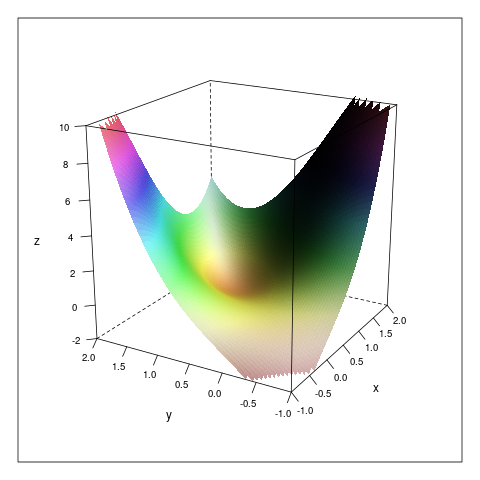
\includegraphics[width=.6\textwidth]{ExempleOptimum-surface}
$$
\paragraph*{Point $a = (0, 0)$:}
$$
\begin{tabular}{cc}
  direction $x = y$ & direction $x = -y$ \\
  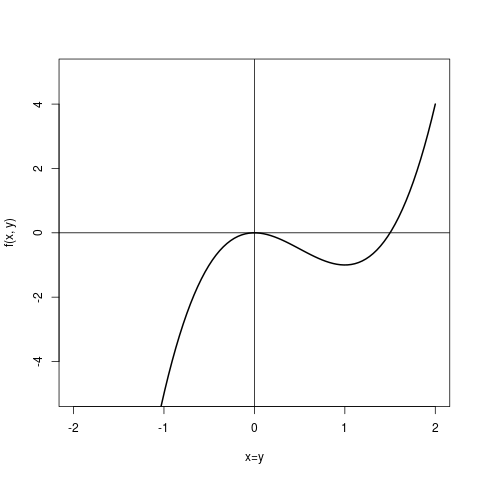
\includegraphics[width=.4\textwidth, trim=10 10 10 40, clip=]{ExempleOptimum-1ereBissectrice} &
  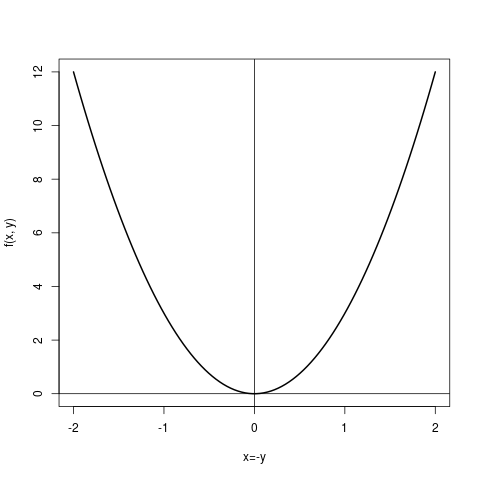
\includegraphics[width=.4\textwidth, trim=10 10 10 40, clip=]{ExempleOptimum-2emeBissectrice} \\
  $f(x, x) = 2x^3 - 3x^2$ & $f(x, -x) = 3x^2$
\end{tabular}
$$
}
